\chapter{Background Knowledge and Related Work}
\label{sec:background}
\begin{itemize}
  \item This chapter provides an overview over key concepts and research relevant for this thesis
  \item the aim is to contextualize the proposed approaches into the current state of research
\end{itemize}


\section{Embeddings}
\label{sec:background:embeddings}
% TODO: add a plot to explain embeddings?
\begin{itemize}
  \item early models learn fixed vectors for words and produce static word embeddings
  \item for example Word2Vec (\cite{mikolovEfficientEstimationWord2013}) and GloVe (\cite{penningtonGloveGlobalVectors2014}) capture semantic similarity from co-occurrence counts
  \item These static embeddings are efficient but ignore word sense variation across contexts
  \item Newer models produce context-dependent vectors (Contextual Word Embeddings)
  \item ELMo (\cite{petersDeepContextualizedWord2018}) uses bidirectional LSTMs to generate embeddings sensitive to surrounding words.
  \item Transformer-based models like BERT (\cite{devlin-etal-2019-bert}) produce deep contextual embeddings
  \item taking the context into account is important because it enables disambiguation of polysemous words and captures nuanced meanings based on usage
  \item for instance, the word \enquote{bank} can refer to a financial institution or the side of a river, and only contextual cues can determine the correct interpretation
  \item contextual embeddings improve performance across a wide range of \ac{nlp} tasks, such as question answering, named entity recognition, and machine translation
  \item these models have led to state-of-the-art results and have become foundational in modern \ac{nlp} pipelines
\end{itemize}


\section{Stylistic Investigations}
\label{sec:background:styleInvestigations}
\begin{itemize}
  \item Stylometric analysis captures writing style independently of content.
  \item Neural methods learn dense style embeddings via proxy tasks (e.g., style transfer, authorship attribution / verification, group membership detection).
        \begin{itemize}
          \item % TODO: write a little more about the proxy tasks; what are they, what are examples, why are they necessary
          \item % TODO: example for learned style embedding method with citation
          \item one disadvantage is that it is difficult to ensure that the embeddings are truly content independent, which makes it more difficult to use them in new domains % TODO: citation?
          \item another disadvantage is that these embeddings are mostly uninterpretable
          \item there are approach to produce interpretable embeddings (\cite{patelLearningInterpretableStyle2023}) or to make embeddings more interpretable (\cite{alshomaryLatentSpaceInterpretation2024})
          \item this thesis presents an extension to the approach to learn interpretable style embeddings
        \end{itemize}
  \item Classical methods use manually selected interpretable features (e.g., function-word frequencies, syntax, punctuation counts). % TODO: citation and/or short explanations what the examples are
        \begin{itemize}
          \item These features enable explainable classifiers but may lack nuance compared to learned embeddings
          \item an example of recent work on the topic of feature extraction is Stylometrix by \citet{okulskaStyloMetrixOpensourceMultilingual2023}, which produces interpretable style vectors where each dimension is a carefully selected feature
          \item another example is StyloAI by \citet{oparaStyloAIDistinguishingAIgenerated2024a}, which extracts \num{31} stylometric features to identify AI-generated texts by applying a Random Forest classifier
          \item advantages:
                \begin{itemize}
                  \item highly relevant features
                  \item high quality of the features and their values
                \end{itemize}
          \item disadvantages:
                \begin{itemize}
                  \item features have to be manually selected
                  \item limited selection of possible features
                  \item it is not possible to include attributes that require text understanding, like knowledge attributes, which are part of the approach presented in this thesis
                \end{itemize}
        \end{itemize}
\end{itemize}


\section{Large Language Models}
\label{sec:background:llm}
% prompting, autoregressiv, token-based
% TODO: rewrite
\begin{itemize}
  \item \Acfp{llm} are large-scale (typically billions of parameters), pre-trained statistical language models based on neural networks
  \item they leverage billions of parameters, which are trained on massive text datasets, to perform tasks which require advanced language understanding and generation (\cite{minaeeLargeLanguageModels2025})
  \item These models have revolutionized NLP by achieving state-of-the-art performance in diverse tasks, including:
        \begin{itemize}
          \item Text generation,
          \item Translation,
          \item Question answering.
        \end{itemize}
  \item Transformer Architecture:
        \begin{itemize}
          \item Introduced by \citet{NIPS2017_3f5ee243} in the paper \textit{Attention Is All You Need}.
          \item Unlike prior models that relied on recurrence or convolution, the Transformer uses self-attention mechanisms.
          \item Enables parallel processing of input data, improving efficiency and scalability especially during training.
          \item Follows an encoder-decoder structure that can be seen in Figure~\ref{fig:transformerArchitecture}:
                \begin{itemize}
                  \item The encoder maps an input sequence to a continuous representation.
                  \item The decoder generates an output sequence conditioned on the encoder's output and its previous outputs.
                \end{itemize}
          \item in this thesis, encoder-only \acp{llm} will be used to create the interpretable attribute embeddings
          \item decoder-only \acp{llm} will be used to generate text
        \end{itemize}
\end{itemize}



\begin{figure}[ht]
  \begin{center}
    % source: https://github.com/negrinho/sane_tikz
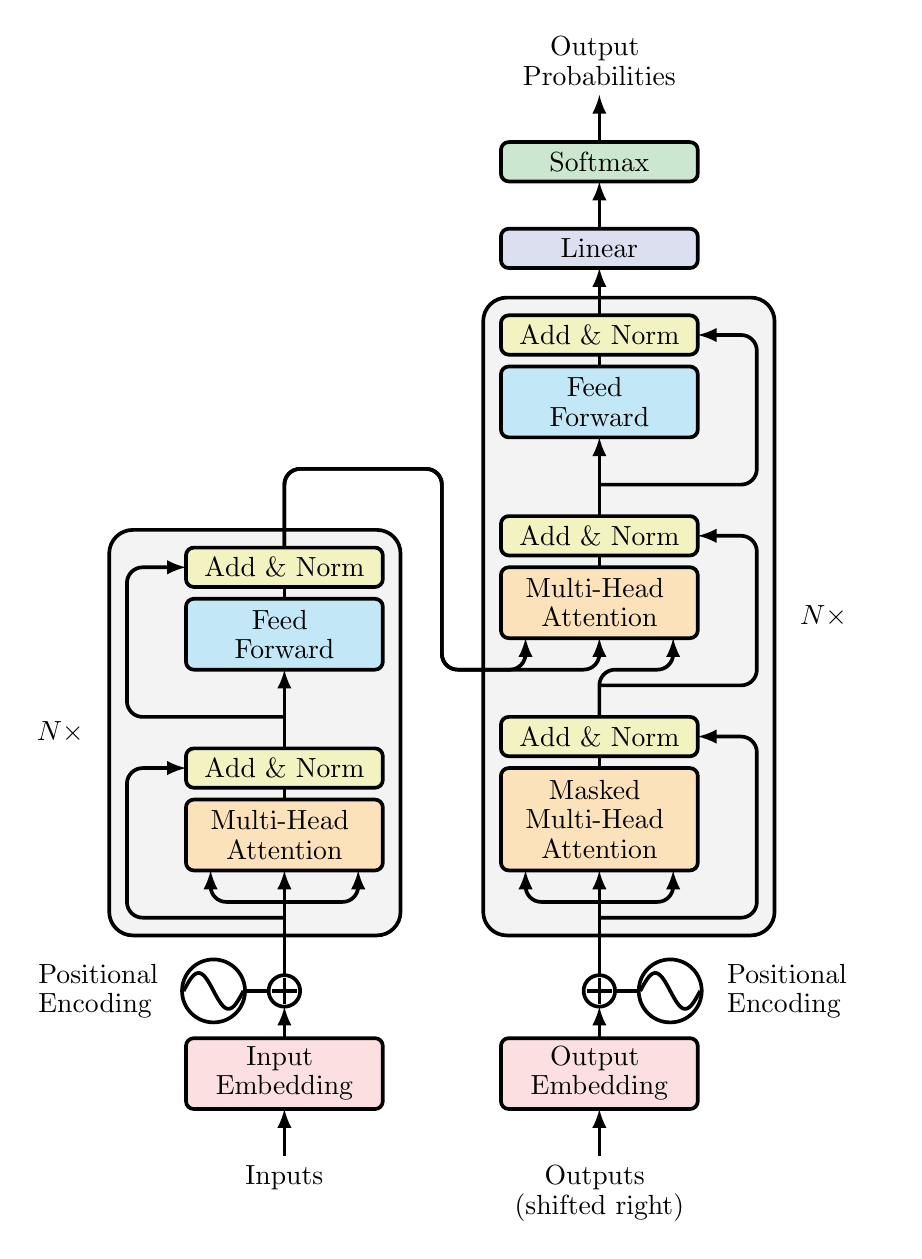
\begin{tikzpicture}
  \definecolor{emb_color}{RGB}{252,224,225}
  \definecolor{multi_head_attention_color}{RGB}{252,226,187}
  \definecolor{add_norm_color}{RGB}{242,243,193}
  \definecolor{ff_color}{RGB}{194,232,247}
  \definecolor{softmax_color}{RGB}{203,231,207}
  \definecolor{linear_color}{RGB}{220,223,240}
  \definecolor{gray_bbox_color}{RGB}{243,243,244}
  \draw[fill=gray_bbox_color, line width=0.046875cm, rounded corners=0.300000cm] (-0.975000, 6.455000) -- (2.725000, 6.455000) -- (2.725000, 1.305000) -- (-0.975000, 1.305000) -- cycle;
  \draw[fill=gray_bbox_color, line width=0.046875cm, rounded corners=0.300000cm] (3.775000, 9.405000) -- (7.475000, 9.405000) -- (7.475000, 1.305000) -- (3.775000, 1.305000) -- cycle;
  \draw[line width=0.046875cm, fill=emb_color, rounded corners=0.100000cm] (0.000000, 0.000000) -- (2.500000, 0.000000) -- (2.500000, -0.900000) -- (0.000000, -0.900000) -- cycle;
  \node[text width=2.500000cm, align=center] at (1.250000,-0.450000) {Input \vspace{-0.05cm} \linebreak Embedding};
  \draw[line width=0.046875cm, fill=emb_color, rounded corners=0.100000cm] (4.000000, 0.000000) -- (6.500000, 0.000000) -- (6.500000, -0.900000) -- (4.000000, -0.900000) -- cycle;
  \node[text width=2.500000cm, align=center] at (5.250000,-0.450000) {Output \vspace{-0.05cm} \linebreak Embedding};
  \draw[line width=0.046875cm, fill=add_norm_color, rounded corners=0.100000cm] (0.000000, 3.680000) -- (2.500000, 3.680000) -- (2.500000, 3.180000) -- (0.000000, 3.180000) -- cycle;
  \node[text width=2.500000cm, align=center] at (1.250000,3.430000) {Add \& Norm};
  \draw[line width=0.046875cm, fill=multi_head_attention_color, rounded corners=0.100000cm] (0.000000, 3.030000) -- (2.500000, 3.030000) -- (2.500000, 2.130000) -- (0.000000, 2.130000) -- cycle;
  \node[text width=2.500000cm, align=center] at (1.250000,2.580000) {Multi-Head \vspace{-0.05cm} \linebreak Attention};
  \draw[line width=0.046875cm] (1.250000, 3.030000) -- (1.250000, 3.180000);
  \draw[line width=0.046875cm, fill=add_norm_color, rounded corners=0.100000cm] (4.000000, 6.630000) -- (6.500000, 6.630000) -- (6.500000, 6.130000) -- (4.000000, 6.130000) -- cycle;
  \node[text width=2.500000cm, align=center] at (5.250000,6.380000) {Add \& Norm};
  \draw[line width=0.046875cm, fill=multi_head_attention_color, rounded corners=0.100000cm] (4.000000, 5.980000) -- (6.500000, 5.980000) -- (6.500000, 5.080000) -- (4.000000, 5.080000) -- cycle;
  \node[text width=2.500000cm, align=center] at (5.250000,5.530000) {Multi-Head \vspace{-0.05cm} \linebreak Attention};
  \draw[line width=0.046875cm] (5.250000, 5.980000) -- (5.250000, 6.130000);
  \draw[line width=0.046875cm, fill=add_norm_color, rounded corners=0.100000cm] (4.000000, 4.080000) -- (6.500000, 4.080000) -- (6.500000, 3.580000) -- (4.000000, 3.580000) -- cycle;
  \node[text width=2.500000cm, align=center] at (5.250000,3.830000) {Add \& Norm};
  \draw[line width=0.046875cm, fill=multi_head_attention_color, rounded corners=0.100000cm] (4.000000, 3.430000) -- (6.500000, 3.430000) -- (6.500000, 2.130000) -- (4.000000, 2.130000) -- cycle;
  \node[text width=2.500000cm, align=center] at (5.250000,2.780000) {Masked \vspace{-0.05cm} \linebreak Multi-Head \vspace{-0.05cm} \linebreak Attention};
  \draw[line width=0.046875cm] (5.250000, 3.430000) -- (5.250000, 3.580000);
  \draw[line width=0.046875cm, fill=add_norm_color, rounded corners=0.100000cm] (0.000000, 6.230000) -- (2.500000, 6.230000) -- (2.500000, 5.730000) -- (0.000000, 5.730000) -- cycle;
  \node[text width=2.500000cm, align=center] at (1.250000,5.980000) {Add \& Norm};
  \draw[line width=0.046875cm, fill=ff_color, rounded corners=0.100000cm] (0.000000, 5.580000) -- (2.500000, 5.580000) -- (2.500000, 4.680000) -- (0.000000, 4.680000) -- cycle;
  \node[text width=2.500000cm, align=center] at (1.250000,5.130000) {Feed \vspace{-0.05cm} \linebreak Forward};
  \draw[line width=0.046875cm] (1.250000, 5.580000) -- (1.250000, 5.730000);
  \draw[line width=0.046875cm, fill=add_norm_color, rounded corners=0.100000cm] (4.000000, 9.180000) -- (6.500000, 9.180000) -- (6.500000, 8.680000) -- (4.000000, 8.680000) -- cycle;
  \node[text width=2.500000cm, align=center] at (5.250000,8.930000) {Add \& Norm};
  \draw[line width=0.046875cm, fill=ff_color, rounded corners=0.100000cm] (4.000000, 8.530000) -- (6.500000, 8.530000) -- (6.500000, 7.630000) -- (4.000000, 7.630000) -- cycle;
  \node[text width=2.500000cm, align=center] at (5.250000,8.080000) {Feed \vspace{-0.05cm} \linebreak Forward};
  \draw[line width=0.046875cm] (5.250000, 8.530000) -- (5.250000, 8.680000);
  \draw[line width=0.046875cm, fill=linear_color, rounded corners=0.100000cm] (4.000000, 10.280000) -- (6.500000, 10.280000) -- (6.500000, 9.780000) -- (4.000000, 9.780000) -- cycle;
  \node[text width=2.500000cm, align=center] at (5.250000,10.030000) {Linear};
  \draw[line width=0.046875cm, fill=softmax_color, rounded corners=0.100000cm] (4.000000, 11.380000) -- (6.500000, 11.380000) -- (6.500000, 10.880000) -- (4.000000, 10.880000) -- cycle;
  \node[text width=2.500000cm, align=center] at (5.250000,11.130000) {Softmax};
  \draw[line width=0.046875cm] (1.250000, 0.600000) circle (0.200000);
  \draw[line width=0.046875cm] (1.410000, 0.600000) -- (1.090000, 0.600000);
  \draw[line width=0.046875cm] (1.250000, 0.760000) -- (1.250000, 0.440000);
  \draw[line width=0.046875cm] (5.250000, 0.600000) circle (0.200000);
  \draw[line width=0.046875cm] (5.410000, 0.600000) -- (5.090000, 0.600000);
  \draw[line width=0.046875cm] (5.250000, 0.760000) -- (5.250000, 0.440000);
  \draw[line width=0.046875cm] (0.350000, 0.600000) circle (0.400000);
  \draw[line width=0.046875cm] (-0.030000, 0.600000) -- (-0.014490, 0.629156) -- (0.001020, 0.657833) -- (0.016531, 0.685561) -- (0.032041, 0.711884) -- (0.047551, 0.736369) -- (0.063061, 0.758616) -- (0.078571, 0.778258) -- (0.094082, 0.794973) -- (0.109592, 0.808486) -- (0.125102, 0.818576) -- (0.140612, 0.825077) -- (0.156122, 0.827883) -- (0.171633, 0.826946) -- (0.187143, 0.822284) -- (0.202653, 0.813971) -- (0.218163, 0.802145) -- (0.233673, 0.786999) -- (0.249184, 0.768783) -- (0.264694, 0.747796) -- (0.280204, 0.724382) -- (0.295714, 0.698925) -- (0.311224, 0.671845) -- (0.326735, 0.643584) -- (0.342245, 0.614608) -- (0.357755, 0.585392) -- (0.373265, 0.556416) -- (0.388776, 0.528155) -- (0.404286, 0.501075) -- (0.419796, 0.475618) -- (0.435306, 0.452204) -- (0.450816, 0.431217) -- (0.466327, 0.413001) -- (0.481837, 0.397855) -- (0.497347, 0.386029) -- (0.512857, 0.377716) -- (0.528367, 0.373054) -- (0.543878, 0.372117) -- (0.559388, 0.374923) -- (0.574898, 0.381424) -- (0.590408, 0.391514) -- (0.605918, 0.405027) -- (0.621429, 0.421742) -- (0.636939, 0.441384) -- (0.652449, 0.463631) -- (0.667959, 0.488116) -- (0.683469, 0.514439) -- (0.698980, 0.542167) -- (0.714490, 0.570844) -- (0.730000, 0.600000);
  \draw[line width=0.046875cm] (6.150000, 0.600000) circle (0.400000);
  \draw[line width=0.046875cm] (5.770000, 0.600000) -- (5.785510, 0.629156) -- (5.801020, 0.657833) -- (5.816531, 0.685561) -- (5.832041, 0.711884) -- (5.847551, 0.736369) -- (5.863061, 0.758616) -- (5.878571, 0.778258) -- (5.894082, 0.794973) -- (5.909592, 0.808486) -- (5.925102, 0.818576) -- (5.940612, 0.825077) -- (5.956122, 0.827883) -- (5.971633, 0.826946) -- (5.987143, 0.822284) -- (6.002653, 0.813971) -- (6.018163, 0.802145) -- (6.033673, 0.786999) -- (6.049184, 0.768783) -- (6.064694, 0.747796) -- (6.080204, 0.724382) -- (6.095714, 0.698925) -- (6.111224, 0.671845) -- (6.126735, 0.643584) -- (6.142245, 0.614608) -- (6.157755, 0.585392) -- (6.173265, 0.556416) -- (6.188776, 0.528155) -- (6.204286, 0.501075) -- (6.219796, 0.475618) -- (6.235306, 0.452204) -- (6.250816, 0.431217) -- (6.266327, 0.413001) -- (6.281837, 0.397855) -- (6.297347, 0.386029) -- (6.312857, 0.377716) -- (6.328367, 0.373054) -- (6.343878, 0.372117) -- (6.359388, 0.374923) -- (6.374898, 0.381424) -- (6.390408, 0.391514) -- (6.405918, 0.405027) -- (6.421429, 0.421742) -- (6.436939, 0.441384) -- (6.452449, 0.463631) -- (6.467959, 0.488116) -- (6.483469, 0.514439) -- (6.498980, 0.542167) -- (6.514490, 0.570844) -- (6.530000, 0.600000);
  \draw[line width=0.046875cm, -latex] (1.250000, 3.680000) -- (1.250000, 4.680000);
  \draw[line width=0.046875cm, -latex] (5.250000, 6.630000) -- (5.250000, 7.630000);
  \draw[line width=0.046875cm, -latex] (5.250000, 9.180000) -- (5.250000, 9.780000);
  \draw[line width=0.046875cm, -latex] (5.250000, 10.280000) -- (5.250000, 10.880000);
  \draw[line width=0.046875cm, -latex] (1.250000, 0.000000) -- (1.250000, 0.400000);
  \draw[line width=0.046875cm, -latex] (1.250000, 0.800000) -- (1.250000, 2.130000);
  \draw[line width=0.046875cm, -latex] (5.250000, 0.800000) -- (5.250000, 2.130000);
  \draw[line width=0.046875cm, -latex] (5.250000, 0.000000) -- (5.250000, 0.400000);
  \draw[line width=0.046875cm] (0.750000, 0.600000) -- (1.050000, 0.600000);
  \draw[line width=0.046875cm] (5.450000, 0.600000) -- (5.750000, 0.600000);
  \draw[-latex, line width=0.046875cm, rounded corners=0.200000cm] (1.250000, 4.080000) -- (-0.750000, 4.080000) -- (-0.750000, 5.980000) -- (0.000000, 5.980000);
  \draw[-latex, line width=0.046875cm, rounded corners=0.200000cm] (1.250000, 1.530000) -- (-0.750000, 1.530000) -- (-0.750000, 3.430000) -- (0.000000, 3.430000);
  \draw[-latex, line width=0.046875cm, rounded corners=0.200000cm] (5.250000, 1.530000) -- (7.250000, 1.530000) -- (7.250000, 3.830000) -- (6.500000, 3.830000);
  \draw[-latex, line width=0.046875cm, rounded corners=0.200000cm] (5.250000, 4.480000) -- (7.250000, 4.480000) -- (7.250000, 6.380000) -- (6.500000, 6.380000);
  \draw[-latex, line width=0.046875cm, rounded corners=0.200000cm] (5.250000, 7.030000) -- (7.250000, 7.030000) -- (7.250000, 8.930000) -- (6.500000, 8.930000);
  \draw[-latex, line width=0.046875cm, rounded corners=0.200000cm] (1.250000, 1.730000) -- (0.312500, 1.730000) -- (0.312500, 2.130000);
  \draw[-latex, line width=0.046875cm, rounded corners=0.200000cm] (1.250000, 1.730000) -- (2.187500, 1.730000) -- (2.187500, 2.130000);
  \draw[-latex, line width=0.046875cm, rounded corners=0.200000cm] (5.250000, 1.730000) -- (4.312500, 1.730000) -- (4.312500, 2.130000);
  \draw[-latex, line width=0.046875cm, rounded corners=0.200000cm] (5.250000, 1.730000) -- (6.187500, 1.730000) -- (6.187500, 2.130000);
  \draw[-latex, line width=0.046875cm, rounded corners=0.200000cm] (1.250000, 6.230000) -- (1.250000, 7.230000) -- (3.250000, 7.230000) -- (3.250000, 4.680000) -- (4.312500, 4.680000) -- (4.312500, 5.080000);
  \draw[-latex, line width=0.046875cm, rounded corners=0.200000cm] (1.250000, 6.230000) -- (1.250000, 7.230000) -- (3.250000, 7.230000) -- (3.250000, 4.680000) -- (5.250000, 4.680000) -- (5.250000, 5.080000);
  \draw[-latex, line width=0.046875cm, rounded corners=0.200000cm] (5.250000, 4.080000) -- (5.250000, 4.680000) -- (6.187500, 4.680000) -- (6.187500, 5.080000);
  \draw[line width=0.046875cm, -latex] (1.250000, -1.500000) -- (1.250000, -0.900000);
  \draw[line width=0.046875cm, -latex] (5.250000, -1.500000) -- (5.250000, -0.900000);
  \draw[line width=0.046875cm, -latex] (5.250000, 11.380000) -- (5.250000, 11.980000);
  \node[text width=2.500000cm, anchor=north, align=center] at (1.250000,-1.500000) {Inputs};
  \node[text width=2.500000cm, anchor=north, align=center] at (5.250000,-1.500000) {Outputs \vspace{-0.05cm} \linebreak (shifted right)};
  \node[text width=2.500000cm, anchor=south, align=center] at (5.250000,11.980000) {Output \vspace{-0.05cm} \linebreak Probabilities};
  \node[anchor=east] at (-1.175000,3.880000) {$N\times$};
  \node[anchor=west] at (7.675000,5.355000) {$N\times$};
  \node[text width=2.000000cm, anchor=east] at (0.250000,0.600000) {Positional \vspace{-0.05cm} \linebreak Encoding};
  \node[text width=2.000000cm, anchor=west] at (6.750000,0.600000) {Positional \vspace{-0.05cm} \linebreak Encoding};
\end{tikzpicture}
  \end{center}
  \caption{TODO:} % TODO: mention source (attention is all you need); explain layers
  \label{fig:transformerArchitecture}
\end{figure}

\subsection{Steering of Large Language Models}
\label{sec:background:llm:steering}
\begin{itemize}
  \item \acp{llm} are very good at text generation
  \item however, often it is important that the generated text follows a specific form or that the model does not produce any toxic or inappropriate responses
  \item for this, there exist multiple steering methods
  \item \textbf{prompt engineering} steers the model by changing the prompt it is presented with during inference, which has the advantage that it does not require any training (\cite{schulhoffPromptReportSystematic2024})
  \item there are many different variations of prompt engineering, with a few techniques explained here:
        \begin{itemize}
          \item the system prompt is a special kind of prompt used in chat-based LLMs to set the model's behavior and tone for an entire session.
                \begin{itemize}
                  \item It is not shown to the user but defines the assistant's persona, goals, constraints, or safety rules.
                  \item For example, it can instruct the model to act as a helpful tutor, follow certain formatting rules, or avoid specific content.
                \end{itemize}
          \item another prompt-based steering method is few-shot prompting, where the task instructions and a few example for solutions for the task are included in the prompt
          \item this enables the model to generalize to similar tasks
                % \item chain-of-thought prompting by Wei et al., 2022 % TODO: include this?
        \end{itemize}
  \item \textbf{fine-tuning} involves updating the model weights on task-specific data
        \begin{itemize}
          \item this is process can yield a strong performance, but it is often too expensive for \acs{llm} as they have billions of parameters that have to be updated
          \item additionally, this approach would require a seperate model for each fine-tuning task to be deployed, which would be a very inefficient use of resources
          \item this motivated parameter-efficient fine-tuning methods, that freeze the weights of the pre-trained \ac{llm} and train just a few layers
          \item examples include prefix-tuning (\cite{liPrefixtuningOptimizingContinuous2021}) where a small continuous task-specific vector (called the prefix) is prepended to the input of the \ac{llm}, which leads to comparable performance to fine-tuning while training only \SI{0.1}{\percent} of the parameters
          \item another example is LoRA (\cite{huLoRALowrankAdaptation2021}), which freezes the parameters of the model and injects parameters that are actually trained. This reduced the amount of trainable weights by the factor \num{10000} with comparable performance to fine-tuning
        \end{itemize}
        % \item \textbf{Reinforcement Learning from Human Feedback (RLHF)} % TODO: include this?
  \item another recent method to steer \acp{llm} is \textbf{activation steering}
        \begin{itemize}
          \item it works by intervening directly in the hidden states of an \acs{llm} to control the text generation
          \item the hidden states are extracted at the end of each layer (see Figure~\ref{fig:transformerArchitecture})
          \item state-of-the-art \acp{llm} have between \num{20} and \num{100} layers, where later layers encode more complex concepts (\cite{bogdanEmergentEffectsScaling2025})
          \item activation steering by extracting hidden states that correspond to specific concepts with one forward pass. These steering vectors are then added to the hidden state of the model during inference to steer it towards this concept (\cite{konenStyleVectorsSteering2024,turnerActivationAdditionSteering2024,subramaniExtractingLatentSteering2022})
        \end{itemize}

\end{itemize}



%%%%%%%%%%%%%%%%%%%%%%%%%%%%%%%%%%%%%%%%%%%%%%%%%%%%%%%%%%%
%%%%%%%%%%%%%%%%%%%%%%%%%%%%%%%%%%%%%%%%%%%%%%%%%%%%%%%%%%%

\section{TODO: remove}
\subsection*{Interpretable Style Representations and Steering in Large Language Models}

\subsubsection{Stylistic Investigations}

Stylometric analysis aims to capture writing **style** independently of content.  Classical approaches use interpretable linguistic features – e.g. function-word frequencies, syntax and punctuation counts – to represent authorial style. These rule-based features enable explainable classifiers (e.g. for authorship or genre) but may lack the nuance of learned representations.  Recent neural methods instead learn dense style embeddings via proxy tasks (such as non-parallel style transfer or authorship verification).  However, Patel et al. (2023) note that such unsupervised neural style embeddings tend to be **uninterpretable**, complicating analysis in high-stakes settings.  To address this, new work seeks **interpretable style vectors**. For example, Patel et al. (2023) generate human-readable style embeddings (LISA) by prompting an LLM on a synthetic stylometry dataset. Similarly, Okulska et al. (2023) introduce *StyloMetrix*, a large set of handcrafted linguistic metrics (grammar, syntax, lexicon) that produce a transparent style-vector for each text. They show these vectors can feed into explainable classifiers and improve tasks like content filtering, genre identification, or authorship attribution.

Handcrafted style features remain competitive in many classification tasks.  Opara et al. (2024) demonstrate this in *StyloAI*: a random-forest classifier using just 31 stylometric features (word lengths, punctuation counts, part-of-speech rates, etc.) can distinguish AI-generated from human text, even outperforming deep neural baselines.  Importantly, such feature-based models reveal which cues the decision relied on.  On the neural side, authorship profiling provides indirect evidence that style can be captured by learned embeddings. Wang et al. (2023) show that embeddings trained to predict an author’s identity are indeed sensitive to writing style (and robust to topic drift).  Building on this, Alshomary et al. (2024) cluster latent document embeddings from an authorship model and then use LLM prompts to label each cluster with stylistic attributes.  The result is a set of human-readable style explanations for each cluster, effectively interpreting the model’s style space.  These studies suggest that, even in opaque deep models, latent vectors can often be linked back to meaningful style features.

Style representations have proven useful for **group-membership classification**.  For instance, Kang et al. (2023) apply stylometric analysis to online peer-support forums and find that user roles can be distinguished by style: senior contributors tend to use more varied emotion words than others, and positive vs. negative emotion usage patterns differ across groups.  In other domains, author profiling (predicting gender, age, etc.) similarly relies on subtle stylistic cues.  Okulska et al. (2023) highlight that their interpretable style vectors “serve two functions: they can be used as input to explainable classification models,” and they empirically improve performance when combined with neural text embeddings.  In summary, the recent literature emphasizes **hybrid approaches** – leveraging both traditional stylometric features and modern embedding-based methods – to build style representations that are both effective for classification and amenable to interpretation.

\subsubsection{Large Language Models}

Large Language Models (LLMs) are typically deep Transformer networks trained to predict token sequences. A standard Transformer block applies multi-head self-attention and feed-forward layers to its inputs.  In practice, many LLMs use a *decoder-only* (autoregressive) architecture: at each step the model computes a probability distribution over the vocabulary for the next token, conditioned on all preceding tokens.  Training is self-supervised: the model maximizes the likelihood of the correct next word given the leftward context, typically via cross-entropy loss over billions of tokens.  Because Transformers process entire sequences in parallel, LLMs can handle extremely long contexts (often thousands of tokens) efficiently.

This pretraining on vast text corpora endows LLMs with broad language knowledge.  For example, Brown et al. (2020) trained GPT-3 with 175 billion parameters and found that simply scaling up allowed **few-shot** learning: the model could perform translation, question-answering, code generation, and even arithmetic without any parameter updates, solely by conditioning on task instructions and examples in the prompt.  Inference in an LLM proceeds by *conditional generation*: the user provides a text prompt (possibly with instructions or examples), and the model generates output token-by-token. Decoding strategies (greedy search, beam search, sampling) convert the token probabilities into text.  Crucially, at each step the model “sees” the entire prompt and all tokens it has already generated, so it can leverage long-range context when choosing the next word.  This mechanism makes LLMs extremely versatile: Jurafsky and Martin (2024) observe that *any* NLP task can be formulated as “predict the next word” given an appropriate prompt. For instance, appending a special token like “tl;dr;” to a news article primes the model to produce a summary in the next tokens.

As a result, LLMs have become the foundation of many NLP applications.  They achieve state-of-the-art or near state-of-the-art on tasks such as summarization, translation, sentiment analysis, question answering, and dialog generation.  In practice, one often uses a single pretrained model (e.g. GPT, PaLM, LLaMA) and applies it to diverse tasks via prompt engineering or lightweight fine-tuning.  The combination of massive scale and flexible generative capability underpins the need for effective *steering* methods (below) to control LLM behavior.

\subsubsection{Steering of Large Language Models}

**Prompt engineering** is the most direct way to steer an LLM.  By carefully crafting the input prompt, one can bias the model toward desired outputs.  Early work showed that providing task instructions and a few exemplars in the prompt – *few-shot prompting* – enables the LLM to generalize to new tasks without any weight updates.  Beyond basic prompting, specialized strategies have been developed.  A notable example is *chain-of-thought prompting* (Wei et al., 2022): exemplars include intermediate reasoning steps, which dramatically improves performance on complex reasoning tasks (e.g. math problems).  Wei et al. report that a 540B-parameter model given just 8 chain-of-thought examples achieves state-of-the-art accuracy on a math benchmark (surpassing even a finetuned baseline).  In practice, prompt engineering now includes techniques like instruction-tuning prompts, question rephrasing, and using system or role-setting prompts to elicit specific styles or constraints.

Beyond zero-shot prompting, LLMs can be steered by adapting their parameters.  **Fine-tuning** involves updating the model weights on task-specific data.  While full fine-tuning can yield strong performance, it is often expensive for very large models.  This has motivated *parameter-efficient* fine-tuning methods.  For example, Li and Liang (2021) introduce *prefix tuning*: they freeze the pretrained LLM and learn a small sequence of continuous vectors (a “prefix”) that is prepended at each layer’s input.  Prefix-tuning achieves performance comparable to full fine-tuning on generation tasks while updating only \~0.1\% of parameters. Other methods like prompt-tuning, adapter layers, and LoRA similarly modify or add a few trainable parameters (often linear or low-rank) to steer the model.  These approaches can be seen as “embedding-based” steering, since they work by learning additional input embeddings or subspace projections rather than altering the core network.

A powerful steering paradigm is **Reinforcement Learning from Human Feedback (RLHF)**.  In RLHF, human annotators provide feedback on model outputs (e.g. ranking or rating them), and this data trains a reward model. The LLM is then fine-tuned via reinforcement learning (e.g. PPO) to maximize this learned reward.  This aligns the model with complex human values (e.g. helpfulness, harmlessness).  Stiennon et al. (2020) applied RLHF to summarization: they collected human preference comparisons of summaries, trained a reward model to predict the preferred summary, and then fine-tuned the LLM with RL. The resulting model produced summaries that human judges preferred even over ground-truth references and those produced by larger supervised baselines.  Similarly, Ouyang et al. (2022) used RLHF to create *InstructGPT*.  Starting from GPT-3, they first fine-tuned on human-written prompts and answers, then collected human rankings of outputs and ran RL.  The final InstructGPT model (even with only 1.3B parameters) generated answers that humans significantly preferred over the original 175B GPT-3, and it reduced toxic or irrelevant outputs.  Today, RLHF (and its variants) is the core technique for aligning chatbots and assistants (e.g. ChatGPT, Anthropic’s models) to user intent and values.

In addition to prompts and weight-tuning, other steering methods manipulate learned representations.  An example is the use of **Concept Activation Vectors (CAVs)** in LLMs.  Zhang et al. (2025) introduce *GCAV*: they train a vector in the model’s activation space that encodes a specific concept (e.g. “toxicity”).  At inference time, they add or subtract this concept vector in selected layers. For instance, removing the “toxicity” vector from hidden states greatly reduces the generation of toxic language.  This lightweight intervention does not require retraining: in fact, GCAV achieves state-of-the-art results on attribute control tasks (toxicity, sentiment, topic, style) simply by adjusting the steering vector and choosing its layer of application.  More generally, these embedding-based controls (soft prompts, prefix vectors, concept vectors) offer a middle ground between surface prompts and full fine-tuning: they steer model behavior via operations on internal or input embeddings, with relatively low computational cost.

\subsubsection{Activation Layer Steering}

Activation (or representation) steering methods intervene directly in an LLM’s internal hidden states to effect control.  One such technique is **activation patching** (a.k.a. *causal tracing*).  Here, some subset of the model’s activations (e.g. of certain neurons or layers) is replaced (“patched”) with values from another input, and the effect on the output is observed.  Zhang and Nanda (2023) formalize this approach: they patch activations in different layers to identify which components causally influence a given behavior.  Their study of “activation patching” provides best-practices for choosing metrics and corruption methods, showing how subtle methodological choices can impact interpretability results.  In essence, activation patching helps localize the neural circuits responsible for a feature (e.g. copying a fact into the answer), and can validate causal hypotheses about model behavior.

A complementary method is **activation addition**.  Subramani et al. (2022) first demonstrated that one can extract a *steering vector* from a pretrained LM by optimizing for a desired output.  Xu et al. (2023) build on this with *Activation Additions (ActAdd)*: given a pair of prompts (one neutral, one expressing the target attribute), they compute the difference of the model’s hidden states. That difference vector – the “steering vector” – is then added to the model’s activations on new inputs to induce the attribute.  Importantly, ActAdd requires no additional training or labels; it simply adds a scaled activation vector at inference time.  Xu et al. show that ActAdd reliably steers outputs across tasks: for example, adding a sentiment steering vector can flip the model’s sentiment, and removing a toxicity vector reduces harmful content. They report state-of-the-art detoxification and sentiment-control on models like GPT-2 and LLaMA-3 using this lightweight method.  Because ActAdd leaves the original model weights untouched, it preserves the base model’s behavior (weights remain interpretable) and isolates the effect of the steering vector.  In fact, ActAdd’s effectiveness suggests that many high-level attributes are latent linear directions in activation space. Subramani et al. (2022) similarly found that adding optimized vectors could force the LLM to output specific target texts (achieving near-perfect control of generation).

Other activation-based methods target concepts or knowledge more explicitly.  Hernandez et al. (2023) study how factual knowledge is encoded in activations and show it can be edited: they identify neurons or attention heads carrying a fact and modify them to change the model’s output (e.g. correcting a false statement). They note that *ablating* attention heads can itself be viewed as a crude form of activation intervention.  Zhang et al. (2025)’s GCAV approach (mentioned above) also falls here: by learning concept vectors for attributes like “toxicity” or “formality” and subtracting them at chosen layers, one directly reshapes the model’s internal representation.  These steering techniques demonstrate that LLM behaviors – from factual recall to writing style – can be manipulated by intervening on internal activations. Such methods offer fine-grained control and insight: they extend the idea of mechanistic interpretability (understanding what each neuron or head does) into an active toolkit for **controlling** model outputs at inference time.

**Sources:** We reviewed recent NLP and ML literature (2020–2025) on style representations (e.g. Patel et al., 2023; Okulska et al., 2023; Kang et al., 2023), transformer-based LLMs (Vaswani et al., 2017; Jurafsky \& Martin, 2024), and LLM steering methods.  Prompt engineering is exemplified by Brown et al. (2020) and chain-of-thought prompting.  Fine-tuning and RLHF are demonstrated by Li \& Liang (2021), Stiennon et al. (2020), and Ouyang et al. (2022).  Activation-level methods include Xu et al. (2023) for activation addition, Zhang \& Nanda (2023) on patching, Subramani et al. (2022) on steering vectors, Hernandez et al. (2023) on knowledge editing, and Zhang et al. (2025) on Concept Activation Vectors. These peer-reviewed sources underscore the emerging trend of interpretable, controllable embeddings and activation interventions in modern NLP.

\section{TODO: remove 2}
\subsection*{Interpretable Style Representations and Steering in Large Language Models}

\subsubsection*{Stylistic Investigations}

\begin{itemize}
  \item Stylometric analysis captures writing \textbf{style} independently of content.
        \begin{itemize}
          \item Classical methods use interpretable features (e.g., function-word frequencies, syntax, punctuation counts).
          \item These features enable explainable classifiers but may lack nuance.
        \end{itemize}
  \item Neural methods learn dense style embeddings via proxy tasks (e.g., style transfer, authorship verification).
        \begin{itemize}
          \item Such embeddings are often \textbf{uninterpretable}.
          \item Patel et al. (2023) propose interpretable style embeddings (LISA) using LLMs and synthetic datasets.
          \item Okulska et al. (2023) introduce \textit{StyloMetrix} – handcrafted linguistic metrics for transparent style vectors.
        \end{itemize}
  \item Handcrafted features remain competitive:
        \begin{itemize}
          \item Opara et al. (2024)'s \textit{StyloAI} uses 31 stylometric features to outperform neural baselines.
        \end{itemize}
  \item Neural authorship profiling:
        \begin{itemize}
          \item Wang et al. (2023): embeddings predict author identity, sensitive to style.
          \item Alshomary et al. (2024): cluster latent embeddings, use LLMs to label clusters with stylistic attributes.
        \end{itemize}
  \item Style helps in group-membership classification:
        \begin{itemize}
          \item Kang et al. (2023): peer-support forums show stylistic cues in user roles.
          \item Okulska et al. (2023): interpretable vectors improve explainability and classification performance.
        \end{itemize}
  \item Emphasis on \textbf{hybrid approaches}:
        \begin{itemize}
          \item Combine traditional stylometric features with modern embeddings.
          \item Achieve interpretable and effective style representations.
        \end{itemize}
\end{itemize}

\subsubsection*{Large Language Models}

\begin{itemize}
  \item LLMs are typically deep Transformer networks (often decoder-only).
        \begin{itemize}
          \item Use self-attention and feed-forward layers.
          \item Trained to predict the next token via cross-entropy loss.
        \end{itemize}
  \item Training on large corpora enables broad capabilities.
        \begin{itemize}
          \item GPT-3 (Brown et al., 2020): 175B parameters, enabled few-shot learning.
        \end{itemize}
  \item Inference via \textit{conditional generation}.
        \begin{itemize}
          \item Decoding strategies: greedy search, beam search, sampling.
          \item Full context is visible at each generation step.
        \end{itemize}
  \item Versatile applications:
        \begin{itemize}
          \item Translation, summarization, sentiment analysis, QA, etc.
          \item Jurafsky and Martin (2024): all NLP tasks can be framed as “predict the next word”.
        \end{itemize}
  \item Prompt engineering and lightweight fine-tuning expand versatility.
\end{itemize}

\subsubsection*{Steering of Large Language Models}
\begin{itemize}
  \item \textbf{Prompt engineering} is the most direct way to steer an LLM.
        \begin{itemize}
          \item Carefully crafted input prompts can bias the model toward desired outputs.
          \item \textit{Few-shot prompting}: providing task instructions and a few exemplars enables generalization to new tasks without weight updates.
          \item Advanced strategies include:
                \begin{itemize}
                  \item \textit{Chain-of-thought prompting} (Wei et al., 2022): uses exemplars with intermediate reasoning steps to boost performance on complex tasks.
                  \item A 540B-parameter model with 8 chain-of-thought examples achieved state-of-the-art math benchmark accuracy.
                \end{itemize}
          \item Other techniques: instruction-tuning prompts, question rephrasing, system/role-setting prompts.
        \end{itemize}

  \item \textbf{Fine-tuning} steers LLMs by adapting their parameters.
        \begin{itemize}
          \item Full fine-tuning yields strong performance but is computationally expensive.
          \item \textit{Parameter-efficient methods}:
                \begin{itemize}
                  \item \textit{Prefix tuning} (Li and Liang, 2021): freezes the model and learns a small sequence of vectors prepended at each layer’s input.
                  \item Achieves performance close to full fine-tuning while updating only $\sim$0.1\% of parameters.
                  \item Other methods: prompt-tuning, adapter layers, LoRA — modify/add a few trainable parameters.
                \end{itemize}
          \item These are \textit{embedding-based} steering techniques.
        \end{itemize}

  \item \textbf{Reinforcement Learning from Human Feedback (RLHF)} is a powerful steering paradigm.
        \begin{itemize}
          \item Human feedback (e.g., ranking outputs) trains a reward model.
          \item LLM is fine-tuned via RL (e.g., PPO) to maximize this reward.
          \item Aligns model with complex human values (e.g., helpfulness, harmlessness).
          \item Examples:
                \begin{itemize}
                  \item \textit{Stiennon et al. (2020)}: used RLHF for summarization, producing outputs preferred over ground-truth and larger baselines.
                  \item \textit{Ouyang et al. (2022)}: created \textit{InstructGPT} — fine-tuned GPT-3 with human-written data and RLHF, outperforming the original 175B GPT-3.
                \end{itemize}
          \item RLHF is central to aligning chatbots (e.g., ChatGPT, Anthropic’s models) to user intent and values.
        \end{itemize}

  \item \textbf{Representation manipulation} is another steering method.
        \begin{itemize}
          \item \textit{Concept Activation Vectors (CAVs)}: manipulate internal model representations.
          \item \textit{GCAV} (Zhang et al., 2025): learns vectors encoding concepts (e.g., toxicity), and adds/subtracts them at inference.
          \item Removes undesired traits (e.g., toxicity) without retraining.
          \item Achieves state-of-the-art on attribute control tasks.
          \item Embedding-based controls (soft prompts, prefix vectors, concept vectors) offer a middle ground between prompting and full fine-tuning.
        \end{itemize}
\end{itemize}

\subsubsection*{Activation Layer Steering}

\begin{itemize}
  \item \textbf{Activation patching} (a.k.a. causal tracing):
        \begin{itemize}
          \item Replace model activations from one input into another to trace causal influence.
          \item Zhang and Nanda (2023): formalize and benchmark activation patching.
        \end{itemize}
  \item \textbf{Activation addition}:
        \begin{itemize}
          \item Subramani et al. (2022): extract steering vectors by optimizing desired outputs.
          \item Xu et al. (2023): \textit{Activation Additions (ActAdd)}:
                \begin{itemize}
                  \item Compute hidden-state difference between attribute-specific and neutral prompts.
                  \item Add the resulting vector to new activations to induce the attribute.
                  \item Requires no training; preserves model weights.
                \end{itemize}
        \end{itemize}
  \item \textbf{Concept/knowledge editing in activations}:
        \begin{itemize}
          \item Hernandez et al. (2023): identify and modify neurons or heads encoding factual knowledge.
          \item GCAV revisited: subtract learned concept vectors (toxicity, formality) to reshape internal representations.
        \end{itemize}
  \item \textbf{Outcome}:
        \begin{itemize}
          \item Enables fine-grained, interpretable, and testable control.
          \item Integrates mechanistic interpretability with active behavioral steering.
        \end{itemize}
\end{itemize}

